\subsection{System Overview}
\label{subsec:overview}

PostureCare is organised as four stages, illustrated in Figure~\ref{fig:architecture}. Each stage
narrows the data: raw frames and sensor samples become continuous signals, signals become discrete
flags, flags that persist become a severity state, and only a bounded subset of severity states
becomes an actual interruption of the user.

\begin{figure}[!ht]
    \centering
    % TODO: replace with the system architecture diagram.
    \framebox[0.9\linewidth][c]{\rule{0pt}{4cm}\textit{Figure placeholder: overall system architecture}}
    \caption{Overall system architecture. Stage 1 acquires frames and physical telemetry, Stage 2
    synchronises them through Firebase, Stage 3 performs qualification and reasoning, and Stage 4
    delivers bounded feedback through the dashboard, speech, and a device indicator.}
    \label{fig:architecture}
\end{figure}

\textbf{Stage 1 -- Edge acquisition.} The Freenove ESP32-S3 captures the video stream from the
OV3660 sensor and samples the ultrasonic rangefinder and photoresistor, publishing raw values to a
Firebase Realtime Database.

\textbf{Stage 2 -- Vision processing and fusion.} A client-side pipeline consumes the video stream
and derives head orientation, Eye Aspect Ratio, blink rate, and a camera-based distance estimate.
These are merged with the physical telemetry into a single ergonomic state.

\textbf{Stage 3 -- Qualification and reasoning.} The fused state is reduced to a set of named
flags; flags are qualified by how long they persist, classified into a severity tier, and, when a
qualified state changes, passed to a cloud LLM for a short context-aware explanation.

\textbf{Stage 4 -- Bounded intervention.} A notification governor decides whether the user is
interrupted at all, through which channel, and how soon the same condition may be raised again.

It should be noted that image data is processed off the microcontroller rather than by an embedded
neural network. This is a deliberate trade-off: it allows the use of a 468-landmark face mesh that
would not fit the device's compute budget, at the cost of transmitting frames off the device, which
carries the privacy implications discussed in Section~\ref{sec:limitations}.

\subsection{Hardware and Sensing}
\label{subsec:hardware}

\subsubsection{Edge Acquisition Module (Freenove ESP32-S3 \& OV3660)}
The edge sensing node is powered by the Freenove ESP32-S3 WROOM module equipped with an integrated
$8\,\text{MB}$ PSRAM and Wi-Fi connectivity. Image streams are captured using an OmniVision OV3660
3-Megapixel camera module \cite{esp32_iot}. The module is mounted at eye level at the top-centre of
the primary monitor; the photoresistor is placed flat on the work surface so that it samples the
light falling on the task area rather than the light reaching the screen bezel.

\begin{figure}[!ht]
    \centering
    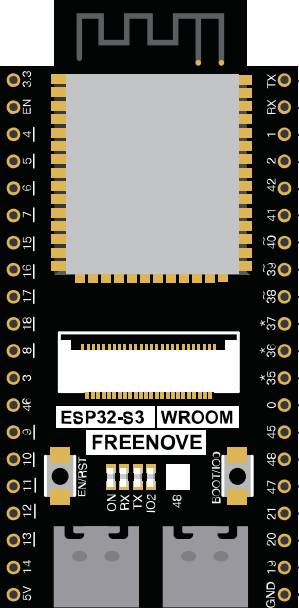
\includegraphics[width=0.22\linewidth]{freenove.png}
    \caption{Freenove ESP32-S3 Board with Integrated Camera Module}
    \label{fig:esp32_s3_board}
\end{figure}

The camera is streamed at QVGA ($320 \times 240$) resolution to keep the wireless link within
budget. This is well below the sensor's native capability and is reported here because the accuracy
of landmark-derived quantities depends on it. In particular, the camera-based distance estimate
(Section~\ref{subsec:vision}) uses a scale factor expressed in pixel units and is therefore
resolution-dependent: changing the capture source invalidates the calibration, which is why
calibration is a mandatory step rather than an optional refinement.

\subsubsection{Multimodal Physical Telemetry Sensors}
\begin{itemize}
    \item \textbf{Eye-to-Screen Distance Telemetry:} An Ultrasonic Sensor (HC-SR04) mounted
    adjacent to the monitor measures real-time distance ($Z_{\text{ultra}}$ in $\text{cm}$) between
    the user and the workstation screen \cite{cvs_distance}.
    \item \textbf{Workspace Illuminance Monitoring:} A Light Dependent Resistor (LDR) module
    collects ambient workspace illuminance levels ($L_{\text{ambient}}$ in $\text{Lux}$)
    \cite{workspace_lighting}.
\end{itemize}

Distance is therefore observed through \emph{two independent channels}: the ultrasonic rangefinder
and the camera-based estimate. This is a cross-validation arrangement rather than redundancy. The
ultrasonic sensor provides a scale reference that does not depend on image geometry, and remains
available when no face is detected; the camera estimate provides continuity when the ultrasonic
returns no echo. The two do not measure the same point --- the rangefinder returns the nearest
surface within its cone, typically the face or chest plane, whereas the camera estimate is
referenced to the interpupillary line --- so their agreement bounds precision rather than
establishing accuracy.

The illuminance channel converts the raw 12-bit ADC reading to lux by inverting the voltage divider
to the photoresistor's own resistance and applying the power-law characteristic of a CdS cell,
which is a straight line in log--log space. Two reference points fully determine that line. The
coefficients used in this work are nominal rather than measured against a photometric reference,
and the consequences are stated in Section~\ref{sec:limitations}.

\subsection{Computer Vision and Ocular Telemetry Pipeline}
\label{subsec:vision}

Instead of on-device embedded neural networks, the vision pipeline leverages a client-side computer
vision stream built on \textbf{MediaPipe} \cite{mediapipe} for spatial posture estimation and
ocular fatigue analysis.

\begin{figure}[!ht]
    \centering
    
\includegraphics[width=0.25\linewidth]{ypr.png}
    \caption{Facial Coordinate Frame Definition for Yaw ($\theta_y$), Pitch ($\theta_p$), and Roll
    ($\theta_r$). Positive pitch corresponds to the head rotating downward toward the desk.}
    \label{fig:ypr_angles}
\end{figure}

\subsubsection{3D Head Pose Estimation via MediaPipe Face Mesh}

\begin{enumerate}
    \item \textbf{Landmark Extraction:} MediaPipe Face Mesh extracts 468 3D facial keypoints from
    the camera feed in real time \cite{mediapipe}.
    \item \textbf{Perspective-n-Point (PnP) Alignment:} Selected 2D landmark coordinates (nose tip,
    chin, outer eye corners, mouth corners) are projected onto a standard 3D facial model using
    OpenCV's \texttt{solvePnP} algorithm \cite{pnp_headpose}.
    \item \textbf{Euler Angle Derivation:} The resulting rotation matrix yields the three canonical
    head orientation angles: Pitch ($\theta_p$), Yaw ($\theta_y$), and Roll ($\theta_r$).
\end{enumerate}

The reported angles are expressed \emph{relative to a per-user zero reference} captured during a
short calibration step at the start of each session, not relative to an anatomical axis. A value of
$\theta_p = 0$ therefore means ``the orientation this user adopted when asked to sit neutrally'',
not ``the cervical spine is in neutral alignment''. This choice follows the personal-calibration
approach reported for webcam posture systems \cite{ref19} and is what makes the angles comparable
within a session; its consequences for interpretation are addressed in
Section~\ref{sec:limitations}.

\subsubsection{Ocular Fatigue \& Blink Frequency Analysis (EAR)}
Visual fatigue is evaluated by computing the Eye Aspect Ratio ($EAR$) using six facial landmarks
per eye \cite{ear_blinking}:

\begin{equation}
EAR = \frac{\|p_2 - p_6\| + \|p_3 - p_5\|}{2 \|p_1 - p_4\|}
\label{eq:ear}
\end{equation}

A blink event is logged when $EAR$ falls below a threshold of $0.294$ for three consecutive frames.
This operating point differs from values commonly quoted in the literature because the magnitude of
Equation~\ref{eq:ear} depends on which landmark indices form the ratio; the present pipeline uses a
specific six-point subset per eye, and the threshold was tuned empirically for that subset rather
than inherited. Blink events are accumulated over a \emph{sliding 60-second window} to yield the
real-time blink rate in blinks per minute, with a warm-up correction of $n/t \times 60$ during the
first minute of a session so that the reported rate reflects current behaviour rather than a
cumulative average.

\subsection{From Signals to Qualified Ergonomic States}
\label{subsec:qualification}

The fused state is expressed as the feature vector $X = [P, D, L, T]$, where $P$ denotes postural
orientation, $D$ viewing distance, $L$ ambient illuminance, and $T$ cumulative exposure. Rather
than mapping $X$ to a single mutually exclusive posture label, the system evaluates each signal
independently and produces a \emph{set} of named flags. This matters because the situations the
system is intended to distinguish are precisely those in which several factors coincide: sitting
close to the screen in a dimly lit room is a different ergonomic condition from either factor
alone, and an exclusive classifier discards exactly that information.

\begin{table}[htbp]
\centering
\caption{Flag vocabulary. Flags in the danger set $D$ qualify after a shorter hold time and are
sufficient on their own to raise the alert tier.}
\label{tab:flags}
\begin{tabular}{@{}llp{6.6cm}@{}}
\toprule
\textbf{Flag} & \textbf{Set} & \textbf{Condition} \\
\midrule
\texttt{head\_too\_low}    & danger & $\theta_p > +5^\circ$ (head rotated down toward the desk) \\
\texttt{head\_too\_high}   & danger & $\theta_p < -5^\circ$ \\
\texttt{head\_tilted}      & danger & $|\theta_r| > 15^\circ$ \\
\texttt{critically\_close} & danger & Viewing distance below $30\,\text{cm}$ \\
\texttt{head\_turned}      & notice & $|\theta_y| > 20^\circ$ \\
\texttt{too\_close}        & notice & Viewing distance below $50\,\text{cm}$ \\
\texttt{too\_far}          & notice & Viewing distance above $70\,\text{cm}$ \\
\texttt{too\_dark}         & notice & Illuminance below $300\,\text{lx}$ \\
\texttt{too\_bright}       & notice & Illuminance above $500\,\text{lx}$ \\
\texttt{low\_blink\_rate}  & notice & Blink rate below $6\,\text{min}^{-1}$ \\
\bottomrule
\end{tabular}
\end{table}

Let $F(t)$ be the set of flags whose condition holds at time $t$:

\begin{equation}
F(t) = \{\, f : \text{condition}_f \text{ holds at } t \,\}
\label{eq:flags}
\end{equation}

A threshold crossing alone is not treated as an ergonomic exposure. Glancing down at the keyboard
produces a momentary crossing that is not equivalent to the same posture sustained for minutes, a
distinction the epidemiological evidence on static loading makes explicitly \cite{ref2,ref12,ref18}.
Each flag must therefore \emph{persist} for a minimum hold time $\tau_f$ before it qualifies:

\begin{equation}
Q(t) = \{\, f \in F(t) : \text{hold}_f(t) \geq \tau_f \,\}
\label{eq:qualify}
\end{equation}

where $\text{hold}_f(t)$ is the elapsed time since flag $f$ last became continuously true, and
$\tau_f$ is $15\,\text{s}$ for the danger set and $60\,\text{s}$ otherwise. The qualified set $Q(t)$
is then mapped to a severity tier:

\begin{equation}
S(t) =
\begin{cases}
\text{escalated} & \text{if the alert tier has held for } \geq 300\,\text{s} \\
\text{alert}     & \text{else if } Q \cap D \neq \emptyset \ \text{ or } \ \texttt{too\_close} \in Q \ \text{ or } \ |Q| \geq 2 \\
\text{notice}    & \text{else if } |Q| = 1 \\
\text{normal}    & \text{otherwise}
\end{cases}
\label{eq:severity}
\end{equation}

The $|Q| \geq 2$ clause is what operationalises the multimodal argument: two individually mild
conditions occurring together are treated as more serious than either alone, without requiring a
trained model to say so.

Postural variables not represented in Table~\ref{tab:flags} were excluded deliberately.
Forward-head displacement, trunk flexion, and slouching are rated of limited feasibility for a
front-facing monocular camera in Table~\ref{tab:posture_variables_detail}, and including them would
have meant reporting quantities the sensing arrangement cannot support.

\subsection{Session Lifecycle and Exposure Measurement}
\label{subsec:session}

Cumulative exposure is only a meaningful variable if it measures time the user actually spent at
the desk. Monitoring is therefore scoped to an explicit session with the states
\textit{idle}, \textit{calibrating}, \textit{monitoring}, \textit{away}, \textit{break}, and
\textit{ended}. Three rules govern the exposure clock:

\begin{itemize}
    \item Exposure accumulates \textbf{only} in the \textit{monitoring} state with a face detected
    --- not merely while the application is open.
    \item Loss of face detection for $30\,\text{s}$ moves the session to \textit{away} and
    \textbf{pauses} the clock. Returning within $180\,\text{s}$ resumes the accumulated total;
    beyond that the exposure counter restarts. A naive timer would otherwise either reset on every
    dropped frame or continue counting an empty chair.
    \item A $20\,\text{s}$ grace period after session start excludes settling-in samples, and those
    samples are marked so that they are also excluded from session-level aggregates.
\end{itemize}

An idle session closes automatically after $900\,\text{s}$ without the user returning. The exposure
measured under these rules is \emph{continuous uninterrupted desk exposure}, which is the quantity
relevant to break-taking guidance. It is not an estimate of daily cumulative sedentary load, and no
claim is made that it maps onto the daily-duration odds ratios reported in Section~\ref{sec:litreview}.

\subsection{Notification Governor}
\label{subsec:governor}

Detecting an unfavourable condition and interrupting the user are different decisions. A system
that raises an alert on every qualified state produces the repetitive generic warnings criticised
in Section~\ref{sec:litreview}, and the practical consequence is that users disable it. The
governor sits between qualification and delivery and applies four rules:

\begin{itemize}
    \item \textbf{Deduplication.} The invocation key is the qualified flag set itself. A condition
    that persists unchanged does not generate a new explanation; a change in the set does.
    \item \textbf{Exponential backoff.} If the same condition remains uncorrected, reminders are
    repeated on a lengthening schedule rather than at a fixed interval. The backoff resets once the
    state has been normal for $120\,\text{s}$, so a later, unrelated violation is still raised
    promptly.
    \item \textbf{Escalation.} An alert sustained for $300\,\text{s}$ escalates and requires
    explicit acknowledgement, which is the design's position on alert fatigue: rather than
    increasing frequency, the system increases salience once and then waits.
    \item \textbf{User control.} Snooze suppresses reminders for $600\,\text{s}$ and a
    do-not-disturb mode suppresses them indefinitely, both reversible from the dashboard.
\end{itemize}

Governor state is persisted with the session record, so cooldowns survive a restart or a second
open dashboard rather than resetting --- without this, a page reload would silently re-enable an
alert the user had just dismissed.

Each delivered reminder additionally opens a $60\,\text{s}$ observation window and records whether
the triggering flags cleared within it. This yields a corrected-per-reminder ratio per session and
is the instrument for the behavioural question posed in Section~\ref{sec:protocol}.

\subsection{Feedback and Intervention Channels}
\label{subsec:feedback}

Interventions are delivered through three channels:

\begin{itemize}
    \item \textbf{Device indication.} The ESP32-S3 drives a two-colour indicator from a state
    object in the Realtime Database: green while monitoring normally, red at the alert tier, and
    blinking red when escalated. Fetching and blinking are non-blocking so that camera streaming
    and sensor sampling are unaffected.
    \item \textbf{Speech.} A single-sentence spoken form of the recommendation is delivered through
    browser speech synthesis. It is opt-in and enabled during guided setup.
    \item \textbf{Interface.} A transient notification carries the governor's available actions
    (snooze, do-not-disturb, acknowledge). A break suggestion is raised when continuous exposure
    reaches its threshold, and is synchronised bidirectionally with the built-in focus timer so
    that a timed break also suspends posture alerting.
\end{itemize}

\subsection{Cloud LLM Integration and Ergonomic Reasoning}
\label{subsec:llm}

The role of the language model \cite{llm_reasoning} is to translate a measured state into an
explanation, not to detect, diagnose, or decide when to interrupt --- those decisions are made by
the deterministic layers above. Invocation is \emph{event-driven}: a request is issued when the qualified flag set
changes, not on a timer. The distinction is material to deployment cost. At the backend's
$10\,\text{s}$ sampling interval, a periodic design would issue on the order of $360$ requests per
hour of sustained poor posture, whereas the governor issues one per distinct condition plus
scheduled repetitions under backoff.

Two bounded prompt modes are used. In \textit{advice} mode the model is constrained to the detected
flags and asked to explain why that combination is unfavourable and what to adjust. In
\textit{explain} mode, used when the user requests an assessment while all readings are in target,
the model is explicitly instructed not to invent a problem. Output follows a fixed
Context/Advice/Spoken contract, the third field being the single short sentence used for speech.

When the API is unavailable the system falls back to a deterministic per-flag phrase table and
labels the resulting record accordingly, so that non-generated text is distinguishable in the logs.

\subsection{Data Schema and Operating Parameters}
\label{subsec:schema}

Table~\ref{tab:data_variables} lists the variables recorded for each sample, and
Table~\ref{tab:parameters} the operating parameters that govern how they are interpreted.

\begin{table}[htbp]
\centering
\caption{Multimodal data variables and system roles}
\label{tab:data_variables}
\begin{tabular}{@{}llp{7.2cm}@{}}
\toprule
\textbf{Variable} & \textbf{Type} & \textbf{Description / Ergonomic Significance} \\
\midrule
Session\_ID        & Categorical & Identifier scoping all rows to one monitoring session \\
Timestamp          & Time        & UNIX timestamp for multi-sensor stream synchronisation \\
State              & Categorical & Session state (idle, calibrating, monitoring, away, break, ended) \\
$\theta_p, \theta_y, \theta_r$ & Continuous & Head orientation Euler angles in degrees ($^\circ$), relative to the calibrated zero \\
EAR                & Continuous & Instantaneous Eye Aspect Ratio \\
Blink Rate         & Continuous & Blink frequency over a sliding 60-second window ($\text{min}^{-1}$) \\
Distance (camera)  & Continuous & Interpupillary-distance estimate of user-to-screen distance (cm) \\
Distance (ultrasonic) & Continuous & Independently measured user-to-screen distance (cm) \\
Light Reading      & Continuous & Workspace ambient illuminance (Lux), with a range status flag \\
Face Present       & Boolean    & Whether a face was detected; gates exposure accumulation \\
Exposure           & Continuous & Continuous uninterrupted desk exposure (s) \\
Flag Set           & Set        & Conditions currently true (Table~\ref{tab:flags}) \\
Flag Durations     & Continuous & Per-flag persistence used by Equation~\ref{eq:qualify} \\
Severity           & Categorical & Tier assigned by Equation~\ref{eq:severity} \\
Reminders / Corrected & Integer & Interventions delivered, and those followed by a correction \\
\bottomrule
\end{tabular}
\end{table}

All operating parameters are read from a single configuration file, so that the values below are
the values the running system uses. Table~\ref{tab:parameters} lists them in full to support
replication.

\begin{table}[htbp]
\centering
\caption{Operating parameters as configured}
\label{tab:parameters}
\begin{tabular}{@{}llp{6.4cm}@{}}
\toprule
\textbf{Parameter} & \textbf{Value} & \textbf{Role} \\
\midrule
\multicolumn{3}{@{}l}{\textit{Detection thresholds}} \\
Pitch                & $\pm 5^\circ$              & Head down / back from calibrated zero \\
Roll                 & $\pm 15^\circ$             & Lateral head tilt \\
Yaw                  & $\pm 20^\circ$             & Rotation away from the screen \\
Viewing distance     & $50$--$70\,\text{cm}$      & Target range \\
Distance, critical   & $< 30\,\text{cm}$          & Distinct acute band \\
Illuminance          & $300$--$500\,\text{lx}$    & Workspace ambient target \\
Blink rate           & $\geq 6\,\text{min}^{-1}$  & Sliding 60\,s window \\
EAR                  & $0.294$ / 3 frames         & Blink event threshold and debounce \\
\midrule
\multicolumn{3}{@{}l}{\textit{Temporal qualification} ($\tau_f$)} \\
Danger flags         & $15\,\text{s}$             & Head-pose and critically-close hold \\
Notice flags         & $60\,\text{s}$             & Lighting, blink rate, distance, head turned \\
Escalation           & $300\,\text{s}$            & Sustained alert without correction \\
\midrule
\multicolumn{3}{@{}l}{\textit{Notification governor}} \\
Backoff              & $60$, $180\,\text{s}$      & Repeat schedule for an unchanged condition \\
Snooze               & $600\,\text{s}$            & User-initiated suppression \\
Normal reset         & $120\,\text{s}$            & Clear time before backoff returns to first step \\
Correction window    & $60\,\text{s}$             & Observation window after a reminder \\
\midrule
\multicolumn{3}{@{}l}{\textit{Session}} \\
Grace                & $20\,\text{s}$             & Post-start settling, excluded from aggregates \\
Face lost $\to$ away & $30\,\text{s}$             & Pause exposure accumulation \\
Away $\to$ reset     & $180\,\text{s}$            & Beyond this, exposure restarts \\
Idle $\to$ end       & $900\,\text{s}$            & Auto-close the session \\
Break suggestion     & $1200\,\text{s}$           & Continuous exposure trigger \\
Sampling interval    & $10\,\text{s}$             & Backend; vision pipeline runs at $\approx$6--7\,Hz \\
\bottomrule
\end{tabular}
\end{table}
